\documentclass[uplatex,12pt]{jsarticle}
\usepackage[dvipdfmx]{graphicx}
\usepackage{url}
\usepackage{listings,jlisting}
\usepackage{ascmac}
\usepackage{amsmath,amssymb}

%ここからソースコードの表示に関する設定
\lstset{
%  basicstyle={\ttfamily},
  basicstyle={\small},
  identifierstyle={\small},
%  commentstyle={\smallitshape},
%  commentstyle={\small\itshape},
  commentstyle={\small\ttfamily},
  keywordstyle={\small\bfseries},
  ndkeywordstyle={\small},
  stringstyle={\small\ttfamily},
  frame={tb},
  breaklines=true,
  columns=[l]{fullflexible},
  numbers=left,
  xrightmargin=0zw,
  xleftmargin=3zw,
  numberstyle={\scriptsize},
  stepnumber=1,
  numbersep=1zw,
  lineskip=-0.5ex
}
%ここまでソースコードの表示に関する設定

\title{知能プログラミング演習II 課題2}
\author{グループ8\\
  29114060 後藤 拓也\\
}
\date{2019年10月28日}

\begin{document}
\maketitle

\paragraph{提出物} rep3

\paragraph{グループ} グループ8

\paragraph{グループメンバー}
\begin{center}
\begin{tabular}{|c|c|c|}
  \hline
  学生番号&氏名&貢献度比率\\
  \hline\hline
  29114003&青山周平&no\\
  \hline
  29114060&後藤拓也&no\\
  \hline
  29114116&増田大輝&no\\
  \hline
  29114142&湯浅範子&no\\
  \hline
  29119016&小中祐希&no\\
  \hline
\end{tabular}
\end{center}
\paragraph{必須課題として} 課題3.1
\\ 「セマンティックネットを構築」
\paragraph{必須課題として} 課題3.2
\\ 「知識をフレームで表現を構築」
\paragraph{自分のメインな役割} 課題3.3
\\ 「知識システムの質問応答システム」
%%%%%%%%%%%%%%%%%%%%%%%%%%%%%%%%%%%%%%%%%%%%%%%%%%%%%%%%%%%%%%%%%%%%%%%%%%%%%%
\section{課題説明}
\subsection{課題3-1}
\begin{screen}
セマンティックネットのプログラムを参考に,自分についてのセマンティックネットを構築せよ.
\end{screen}
\subsection{課題3-2}
\begin{screen}
フレームのプログラムを参考に,自分の興味分野に関する知識をフレームで表現せよ.その分野の知識を表す上で必須となるスロットが何かを考え,クラスフレームを設計すること.
\end{screen}
\subsection{課題3-3}
\begin{screen}
課題3-1または3-2で作った知識表現を用いた質問応答システムを作成せよ.
なお,ユーザの質問は英語や日本語のような自然言語が望ましいが,難しければ課題2で扱ったような変数を含むパターン (クエリー) でも構わない.
\end{screen}
\\\\\\\\\\\\\\\\
\section{手法}
\subsection{課題3-1}
セマンティックネットを構築するためのデータとして以下のようなデータをsemantic\_net/members/下に用意した.
\begin{lstlisting}[caption=semantic\_net/members/goto.txt, label=mid]
Saxphone is-a Instrument
Gotaku is-a NIT-student
Gotaku joins NitWindOrchestra
Gotaku hobby Saxphone
NyankoGreatWar is-a game
game has-a story
Gotaku plays NyankoGreatWar
NIT-student is-a student
student do study
Aladdin is-a animation
Gotaku watches Aladdin
Aladdin is-a Disney
Disney is Fantasy
\end{lstlisting}


上記のセマンティックネットの概念図は以下のようになる.

\begin{figure}[htbp]
 \begin{center}
  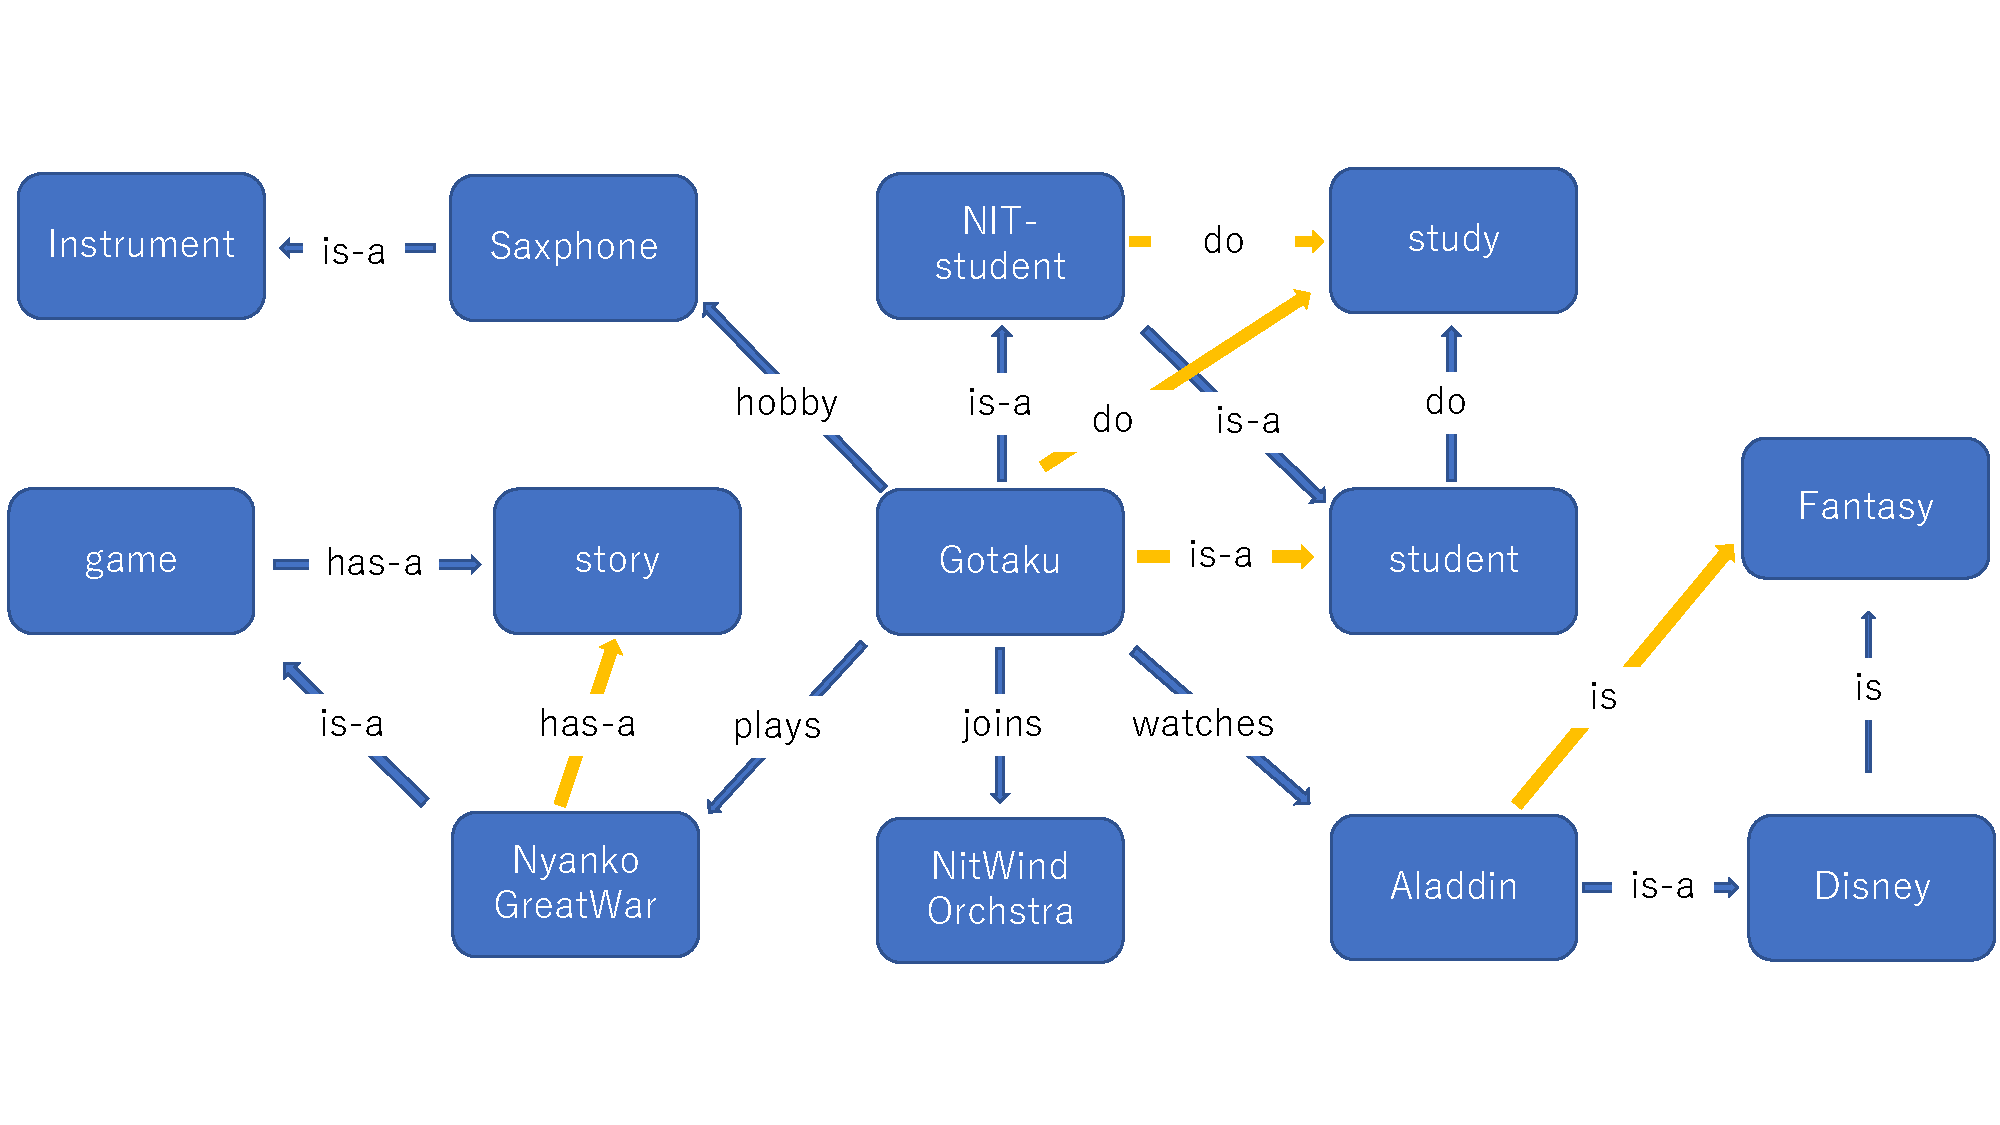
\includegraphics[width = 11cm, pagebox = cropbox, clip]{goto_semantic_net.pdf}
 \end{center}
 \caption[]{セマンティックネットの概念図}\label{fig:fig1.1}
\end{figure}

クエリによる検索を行うための以下のデータをsemantic\_net/queries/下に用意した.\\

\begin{lstlisting}[caption=semantic\_net/queries/goto.txt, label=mid]
?y plays NyankoGreatWar
?y is-a student
?y watches Aladdin
\end{lstlisting}
\subsection{課題3-2}
フレームを構築するためのデータとして,以下のデータをframe/games/下に用意した.
\begin{lstlisting}[caption=frame/games/Pawapuro-Kun.txt, label=mid]
3DS
9400
500
9900
\end{lstlisting}

上記のインスタンスフレームであるPawapuro-Kunフレームの図を示す.
\begin{figure}[htbp]
 \begin{center}
  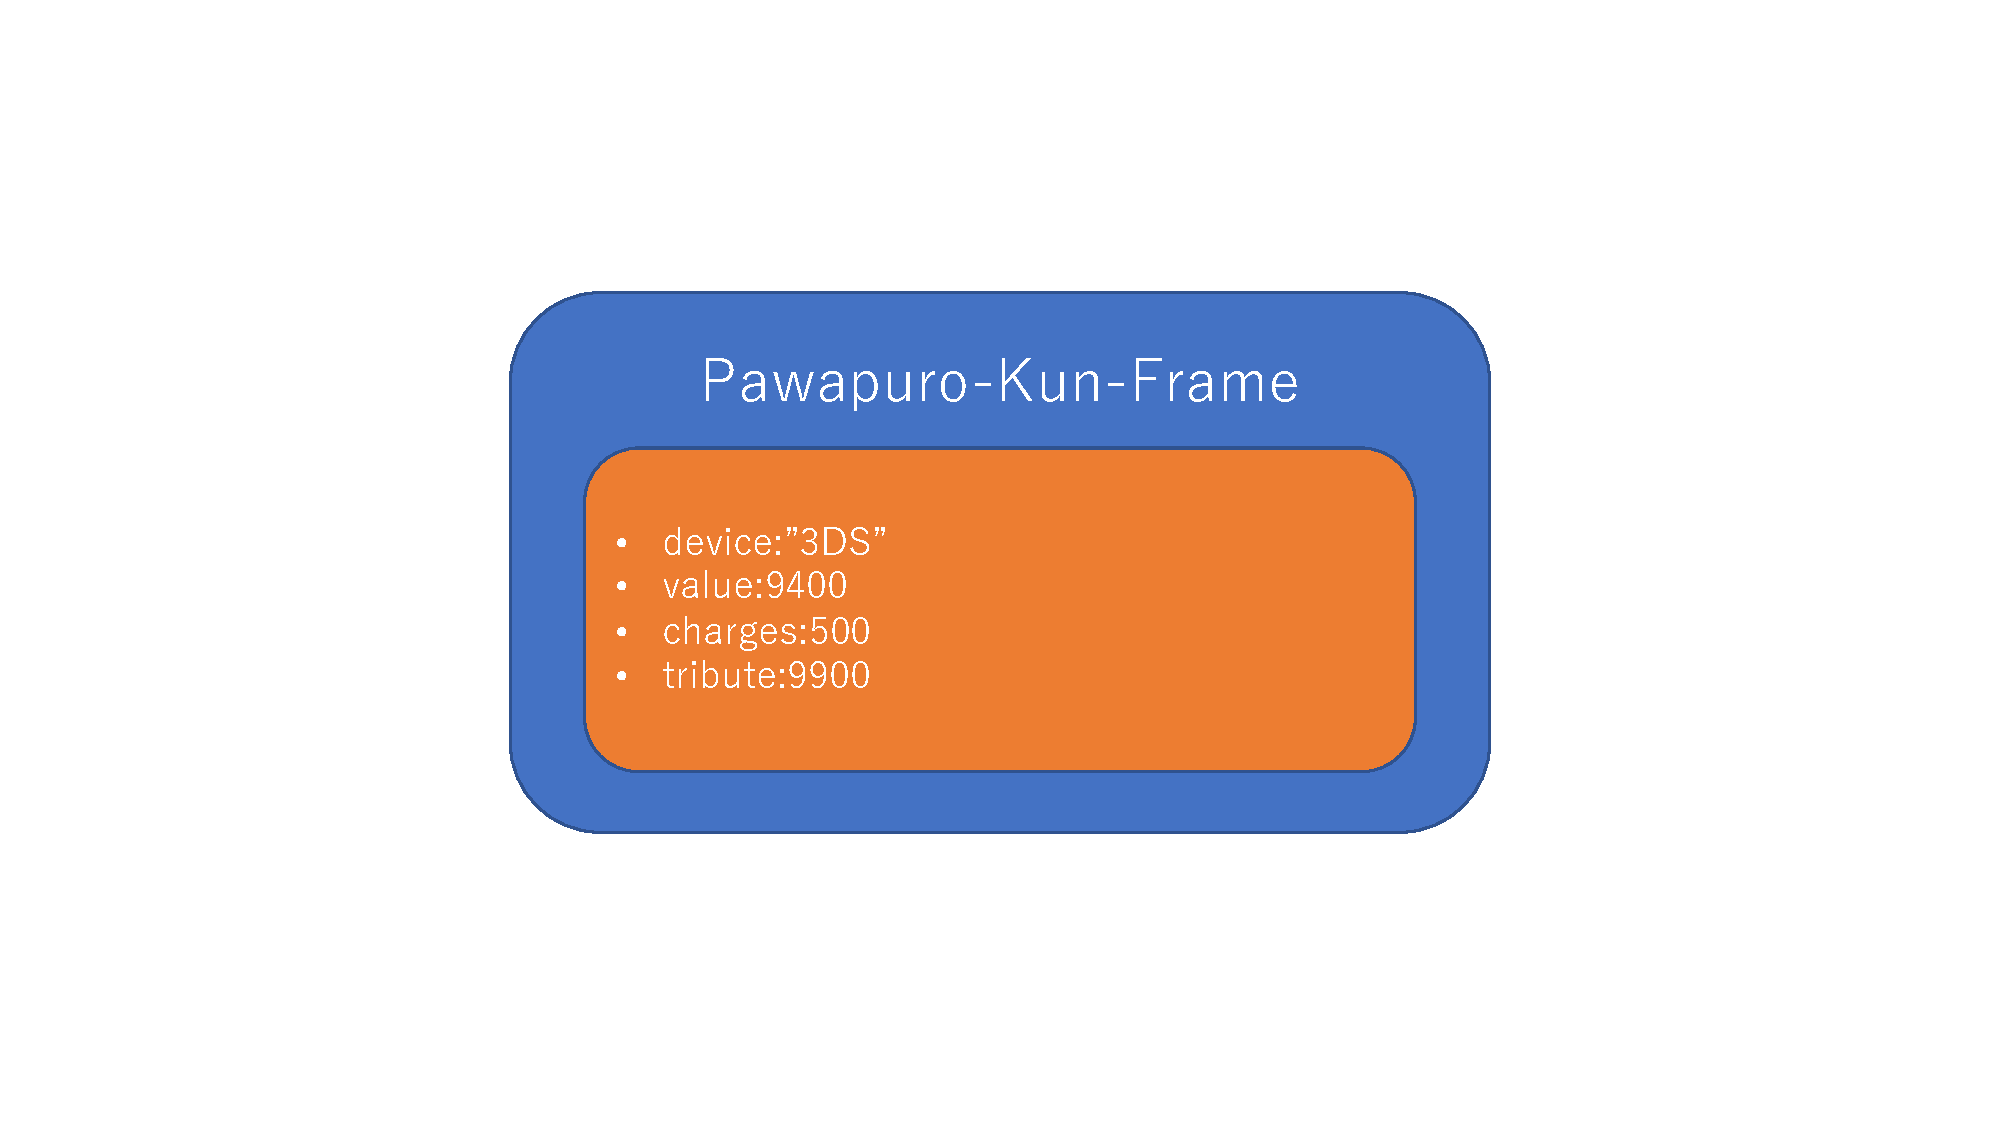
\includegraphics[width = 12cm, pagebox = cropbox, clip]{pawaporo_kun_frame.pdf}
 \end{center}
 \caption[]{フレームの概念図}\label{fig:fig1.1}
\end{figure}

\subsection{課題3-3}
課題3-3の手法として以下の2つを用いた.

\begin{enumerate}
\item 課題2で扱ったような変数を含むクエリーによる質問
\item 英文による質問
\end{enumerate}

\subsubsection{手法1に関して}
変数(?xや?yなど)を含み, [Tail, Label, Head]の形を守って代入する. 具体的には「Taro hobby baseball」という英文ではなく, 単なるクエリーに対して, 「Taro hobby ?x」といったクエリーの形に添った質問をするといった手法である.

\subsubsection{手法2に関して}
ある一定の知識システムが構築された状態において, 質問する内容というのは自ずと限られてくる. 今回は質問とそれに基づく応答を大きく以下の2パターンに分けている. 

\begin{enumerate}
\item 疑問詞Whatに基づく質問から,  ?xの内容を答える
\item 質問の内容に対して, YesかNoかで答える
\end{enumerate}

1. の疑問詞を含む質問に関しては, 質問の内容からどのようにHead, Tail, Labelを取り出すかは, 以下の図1を参照してほしい.
\begin{figure}[htbp]
 \begin{center}
  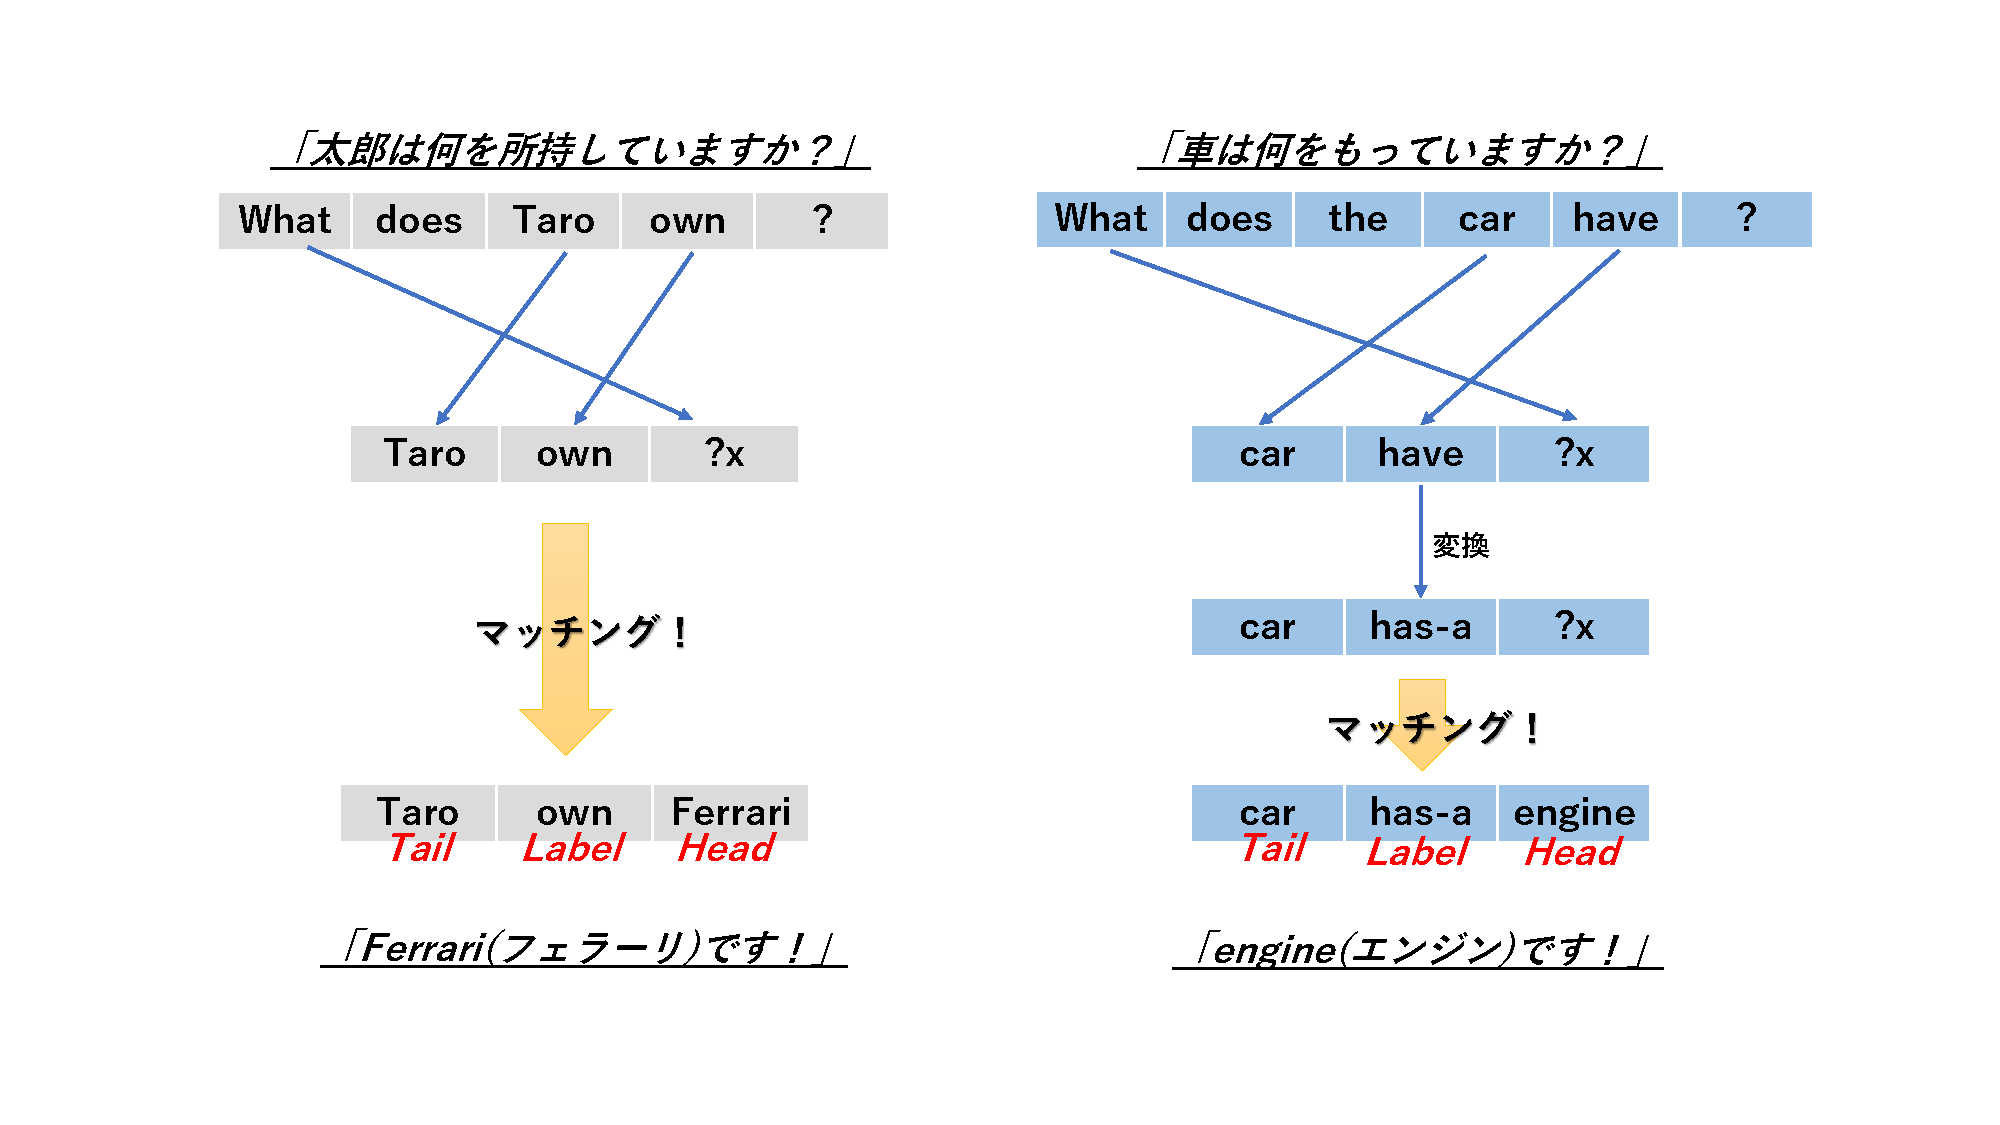
\includegraphics[width = 9cm, pagebox = cropbox, clip]{英文構造_疑問詞SVO.pdf}
 \end{center}
 \caption[]{SVO構造による疑問詞の質問}\label{fig:fig1.1}
\end{figure}

英語の第3文型SVO型は, S(主語)がTail, V(動詞)がLavel, 0(目的語)がHeadになっている. その形に沿って, 疑問文から要素を抽出する. もちろん, 前置詞の処理や, haveをhas-a関係に合わせるなどの調整も必要である.

この質問は"Whatを使って問われる内容は, 目的語の部分のみ"というのを暗示している. 「車はエンジンを持つ」という1文が存在する際に, 「車は何を持ちますか?」とは聞けても, 「エンジンを持っているのは何ですか」とは聞けない. \\

2. のYesかNoで答える質問に関しても, 以下の図2のように分解できる.
\begin{figure}[htbp]
 \begin{center}
  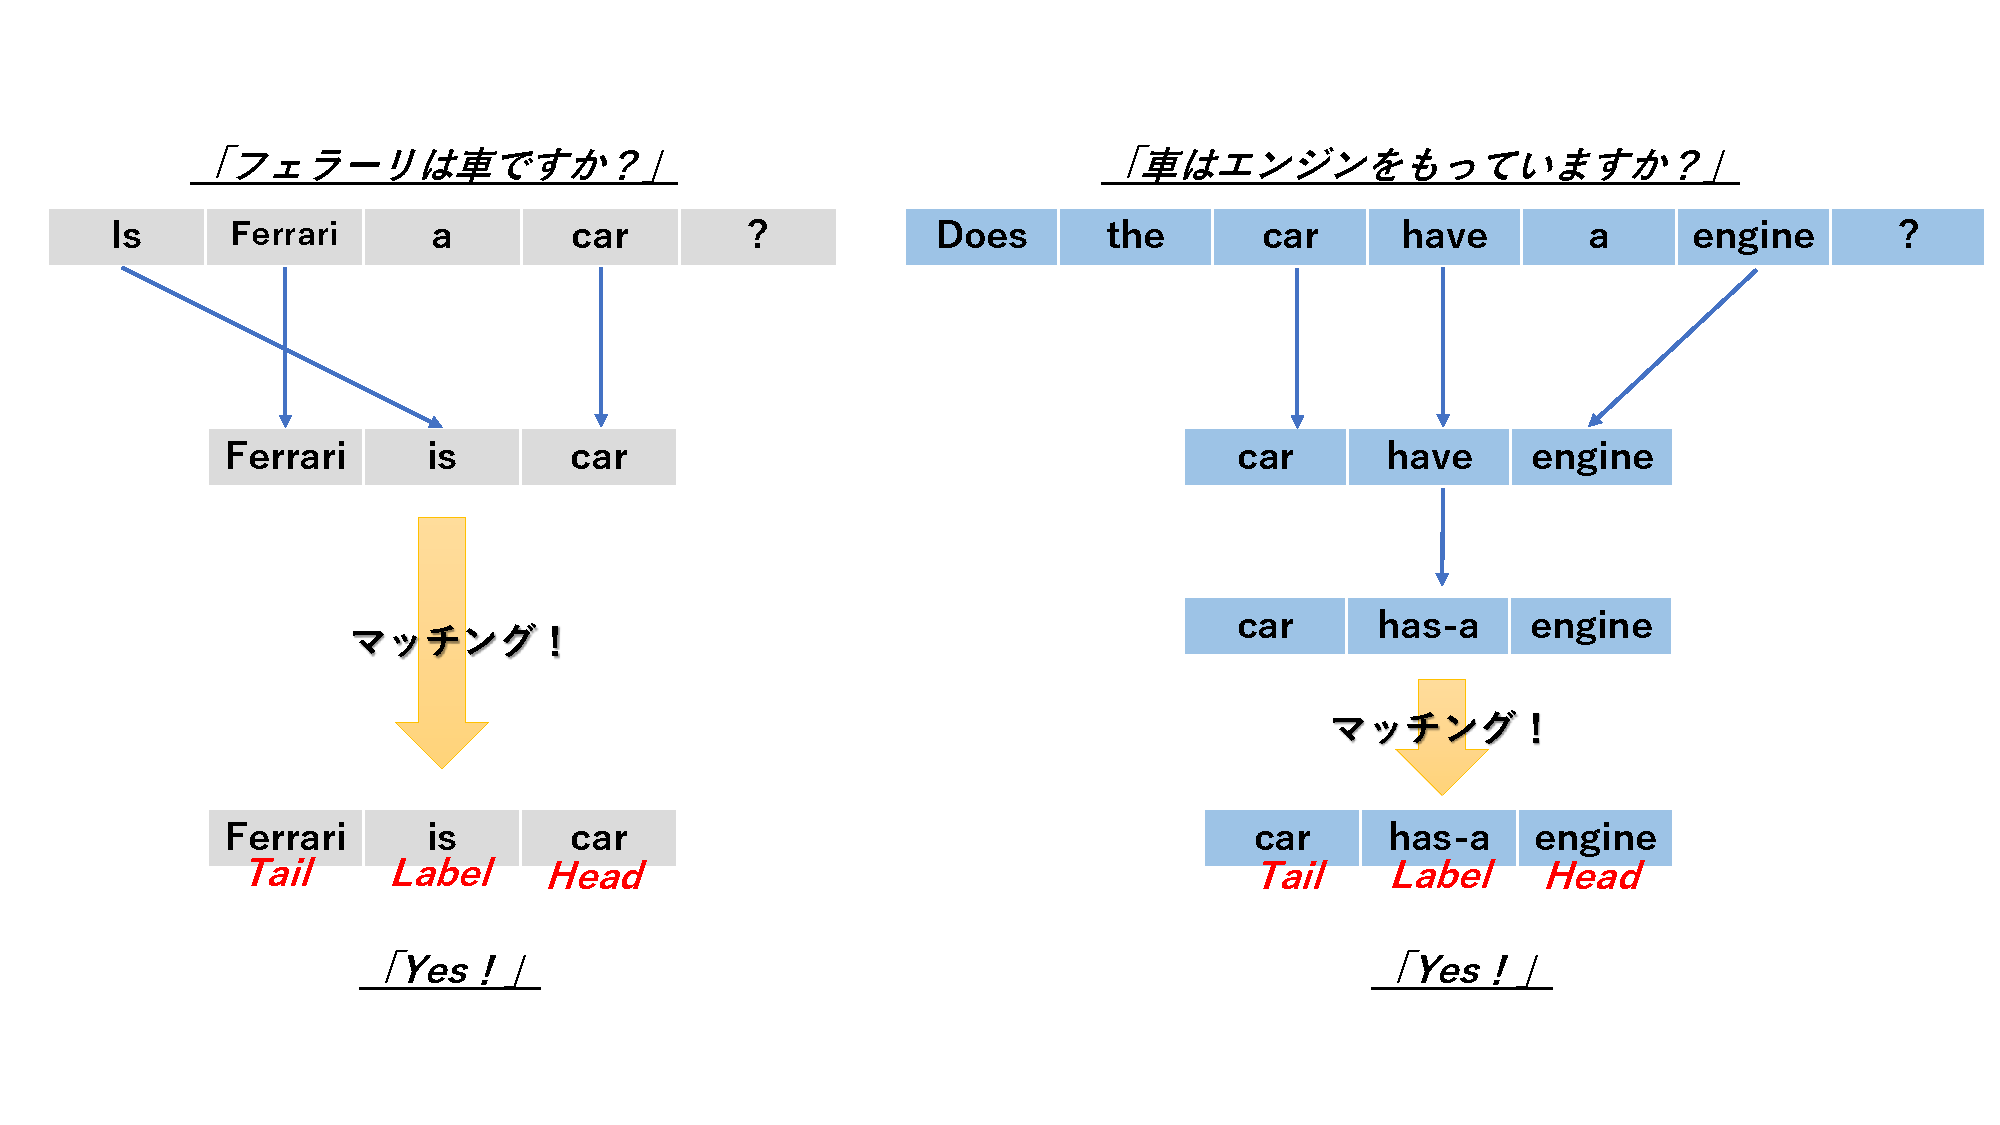
\includegraphics[width = 9cm, pagebox = cropbox, clip]{英文構造_YesNo型.pdf}
 \end{center}
 \caption[]{Yes/Noで答える型}\label{fig:fig1.1}
\end{figure}

 同様にSVCをそれぞれTail, Lavel, Headに合わせ, マッチングが成功したら, 「Yes」を返し, 失敗した場合は「No」を返す.

そして, だれもが違和感を覚えたのは, 「Taro hobby baseball」という1文. 何となく「太郎の趣味は野球です」になるが, Google翻訳にかけたら, 「ヒロキホビーサッカー」である. そもそもhobbyは動詞になり得ない. 正しくは, 「Taro's hobby is baseball」である. これに質問をするには, 「Is Taro's hobby a baseball ?」に対応する必要がある. そのため, 図2のようなLabelの取り方ではいけない. 質問において, 2つ目のトークンに「's」があるかどうかで処理を変える.

\section{実装}
\subsection{課題3-1}
semantic\_net/下においてコンパイル後に以下のコマンドを実行することで対象のテキストファイルに含まれるデータのセマンティックネットを構築できる. \\
java SemanticNetTest [名前] 
\subsection{課題3-2}
frame/下においてコンパイル後に以下のコマンドを実行することで対象のテキストファイルに含まれるデータのフレームを構築できる. \\
java FrameTest [ゲーム名] 

\subsection{課題3-3}
\subsubsection{手法1}
まずは, 手法1に関する「課題2で扱ったような変数を含むクエリーによる質問」の部分を実装したソースコード\ref{src:No1}に示す。
\begin{lstlisting}[caption=クエリーの形に添った質問応答, label=src:No1]
/***
 * 課題2で扱ったような変数を含むパターン (クエリー)による質問応答システム
 * "?x is-a sports"と"?y hobby ?x"をとらえる
 * → 質問は3つのトークンに分けられる
 */
Scanner stdIn1 = new Scanner(System.in);	//文字列読み込み
Scanner stdIn2 = new Scanner(System.in);	//数値読み込み
ArrayList<ArrayList<String>> queryList 
    = new ArrayList<ArrayList<String>>(); //質問(query)を入れる
StringTokenizer st;		//トークンごとに分解
int retry;
do {
	ArrayList<String> tokenList = new ArrayList<>();
	System.out.println("質問を入力してください");
	String s = stdIn1.nextLine(); 	//質問文がここに入り,
	st = new StringTokenizer(s);	//トークンごとに分解し,
	for(int i=0; i<st.countTokens(); i++) {
		tokenList.add(st.nextToken());
	}
	tokenList.add(st.nextToken());
	queryList.add(tokenList);
	System.out.println("もう1つ? 1...Yes/ 0...No");
	retry = stdIn2.nextInt();
}while(retry == 1);

ArrayList<Link> query = new ArrayList<Link>();
for(int i=0; i<queryList.size(); i++) {
	query.add(new Link(queryList.get(i).get(1), queryList.get(i).get(0), queryList.get(i).get(2)));
}
sn.query(query);
\end{lstlisting}

上記のプログラムはmain文において, 全てのリンクをSemanticNetクラスのインスタンスに加えて後で行われ, その後, queryメソッドを呼び出している. 質問文はJavaの文字列読み込みのScannerクラスを用いている. それにより入力されたString型のデータを空欄があるたびに分割するStringTokenizerを利用して各トークンに分け, それぞれを適切にTail, Label, Headに分け, queryメソッドを呼び出している.

\subsubsection{手法2}
次に, 「英語の質問応答システム」の条件分岐の部分をソースコード\ref{src:No2}に示す.
\begin{lstlisting}[caption=英語における質問応答, label=src:No2]
	ArrayList<String> tokenList = new ArrayList<>();
	System.out.println("質問を入力してください");
	String s = stdIn1.nextLine(); 	//質問文がここに入り,
	st = new StringTokenizer(s);	//トークンごとに分解し,

	String firstToken = st.nextToken();
	String secondToken = st.nextToken();
	if(firstToken.equals("What")) {
		if(secondToken.equals("does")) {
			String thirdToken = st.nextToken();
			if(thirdToken.equals("the")) 
				thirdToken = st.nextToken();
			tokenList.add(thirdToken);
	
			String forthToken = st.nextToken();
			if(forthToken.equals("have"))
				tokenList.add("has-a");
			else
				tokenList.add(forthToken);
			tokenList.add("?x");
		}
		else if(secondToken.equals("is")) {
			String thirdToken = st.nextToken().replace("'s", "");
			tokenList.add(thirdToken);
			tokenList.add(st.nextToken());
			tokenList.add("?x");
		}
	}
	else if(firstToken.equals("Is")) {
		if(secondToken.contains("'s")) {
			tokenList.add(secondToken.replace("'s", ""));
					・
					・	   		//以下"Is"における"Yes, No返答"の
					・			//細かい条件分岐が行われている.

\end{lstlisting}

各トークンのメソッドを参照するnextTokenメソッドは呼び出すたびに, 次のトークンへ参照先が移ってしまうので, 条件分岐をする際には, firstToken, secondTokenのように一度String型に格納している. \ref{src:No2}の最初のif文では, 手法2で述べた1つ目の応答パターン「疑問詞Whatに基づく質問」の詳細と, 2つ目の応答パターン「Yes, Noで答える質問」の冒頭が示されている. 疑問詞Whatの後には, SVO関係の場合には"does"が, SVC構文の時には"is"とさらに2パターンに分かれている. 前置詞theを飛ばしたり, haveをhas-aに変更するなどを行う. 

ここでポイントになるのは, 質問文には必ず"(空欄) + ?"を入れてもらいたいということだ. というのも, nextTokenメソッドは呼び出し後に次のトークンを参照するので, もし"(空欄) + ?"がなければ, 文を最後まで参照した後に, 参照する次のトークンがなくなってしまい, エラーになってしまうからである.

\section{実行例}
\subsection{課題3-1}
次に, "java SemanticNetTest goto"の実行例を示す.
\begin{lstlisting}[caption=java SemanticNetTest gotoの実行例, label=mid]
~/Programming2/Work3/semantic_net
●java SemanticNetTest goto                                                                                                                                                                                             【 fix/semantic_net 】
*** Links ***
Saxphone  =is-a=>  Instrument
Gotaku  =is-a=>  NIT-student
Gotaku =joins=> NitWindOrchestra
NyankoGreatWar  =is-a=>  game
game  =has-a=>  story
( NyankoGreatWar  =has-a=>  story )
Gotaku  =plays=>  NyankoGreatWar
NIT-student  =is-a=>  student
( Gotaku  =is-a=>  student )
student  =do=>  study
( NIT-student  =do=> study  )
( Gotaku  =do=>  study )
Aladdin  =is-a=>  animation
Gotaku  =watches=>  Aladdin
Aladdin  =is-a=>  Disney
Disney  =is=>  Fantasy
( Aladdin  =is=>  Fantasy )
*** Nodes ***
Saxphone
Instrument
Gotaku
NIT-student
NitWindOrchestra
NyankoGreatWar
game
story
student
Aladdin
animation
Disney
Fantasy
*** Query ***
?y  =plays=>  NyankoGreatWar
?y  =is-a=>  student
?y  =watches=>  Aladdin
[{?y=Gotaku}]
\end{lstlisting}

\subsection{課題3-2}
次に,"java FrameTest Pawapuro-Kun"の実行例を示す.
\begin{lstlisting}[caption=java FrameTest Pawapuro-Kunの実行例, label=mid]
~/Programming2/Work3/frame
●java FrameTest Pawapuro-Kun                                                                                                                                                                                                  【 fix/frame 】
クラスフレーム:game
インスタンスフレーム:Pawapuro-Kun
device,value,charges,tribute はデフォルト値
スロット値一覧
device:device
value:0
charges:0
tribute:0
tribute はデフォルト値
スロット値一覧
device:3DS
value:9400
charges:500
tribute:9900
再びデフォルト値
スロット値一覧
device:device
value:0
charges:0
tribute:9900
\end{lstlisting}

\subsection{課題3-3}
\subsubsection{手法1}
日本語で言うと, [スポーツを趣味にしている人はだれか?]と質問したときの実行結果が以下のようになる.
\begin{lstlisting}
Successfully started
検索結果を取得
質問を入力してください
?x is-a sports
もう1つ? 1...Yes/ 0...No  1
質問を入力してください
?y hobby ?x
もう1つ? 1...Yes/ 0...No  0
*** Query ***
?x  =is-a=>  sports
?y  =hobby=>  ?x
[{?x=baseball, ?y=Taro}]
\end{lstlisting}

まずはスポーツが何か(?x)を求め, その後, そのスポーツに該当する何か(?y)を趣味としている人を探す. 正しい関係性が出力されていることが確認される.

ここで注目したいのは, 1回の実行における複数の質問内容は"かつ"の条件で結ばれているということである. これはソースコード\ref{src:No1}をみるとわかることだが, do-whileでループさせることで, queryメソッドに入れる内容が増え, SemanticNetクラスのqueryLinkメソッドで, 新しいリンクが構築されていくからである.

\subsubsection{手法2}
\begin{lstlisting}
質問を入力してください
What is Taro's speciality ?
*** Query ***
Taro  =speciality=>  ?x
{?x=AI}です.
もう1回? 1...Yes/ 0...No 1
質問を入力してください
Is Taro a NIT-student ?
*** Query ***
Taro  =is-a=>  NIT-student
Yes!
もう1回? 1...Yes/ 0...No 1
質問を入力してください
Is Taro a student ?
*** Query ***
Taro  =is-a=>  student
Yes!
\end{lstlisting}

適切な英語で質問をすることで, 結果が返ってくる. Goole翻訳を使うことをお勧めする. 上記の例では, 「太郎はNITの生徒」と「生徒は勉強しない」から「太郎は勉強しない」がうまく結果として出力されていることがわかる.

また, 手法1とは異なり, "かつの関係"をもって複数の質問をする機能はつけていない. 入力した1つ質問に対して, 1つの答えが出力される. 

\section{考察}
課題3-3を扱っていく中で, 気になる点があった. 次にはその点について, 英語で質問をした際の答えの出力結果を示す.
\begin{lstlisting}
質問を入力してください
Does Taro own a car ?
*** Query ***
Taro  =own=>  ?x
{?x=Ferrari}です.
もう1回? 1...Yes/ 0...No 1
質問を入力してください
Is Ferrari a car ?
*** Query ***
Ferrari  =is-a=>  car
Yes!
もう1回? 1...Yes/ 0...No 1
質問を入力してください
Does Taro own car ?
*** Query ***
Taro  =own=>  car
No...
\end{lstlisting}

文章的には, 「太郎はフェラーリを持っていて, フェラーリは車なのだから, 太郎は車をもっている」と思うが, このプログラムの継承の仕方ではうまくいかない. 継承にはLabel名が関わっているのである. 以下の図を見てもらいたい.
\begin{figure}[htbp]
 \begin{center}
  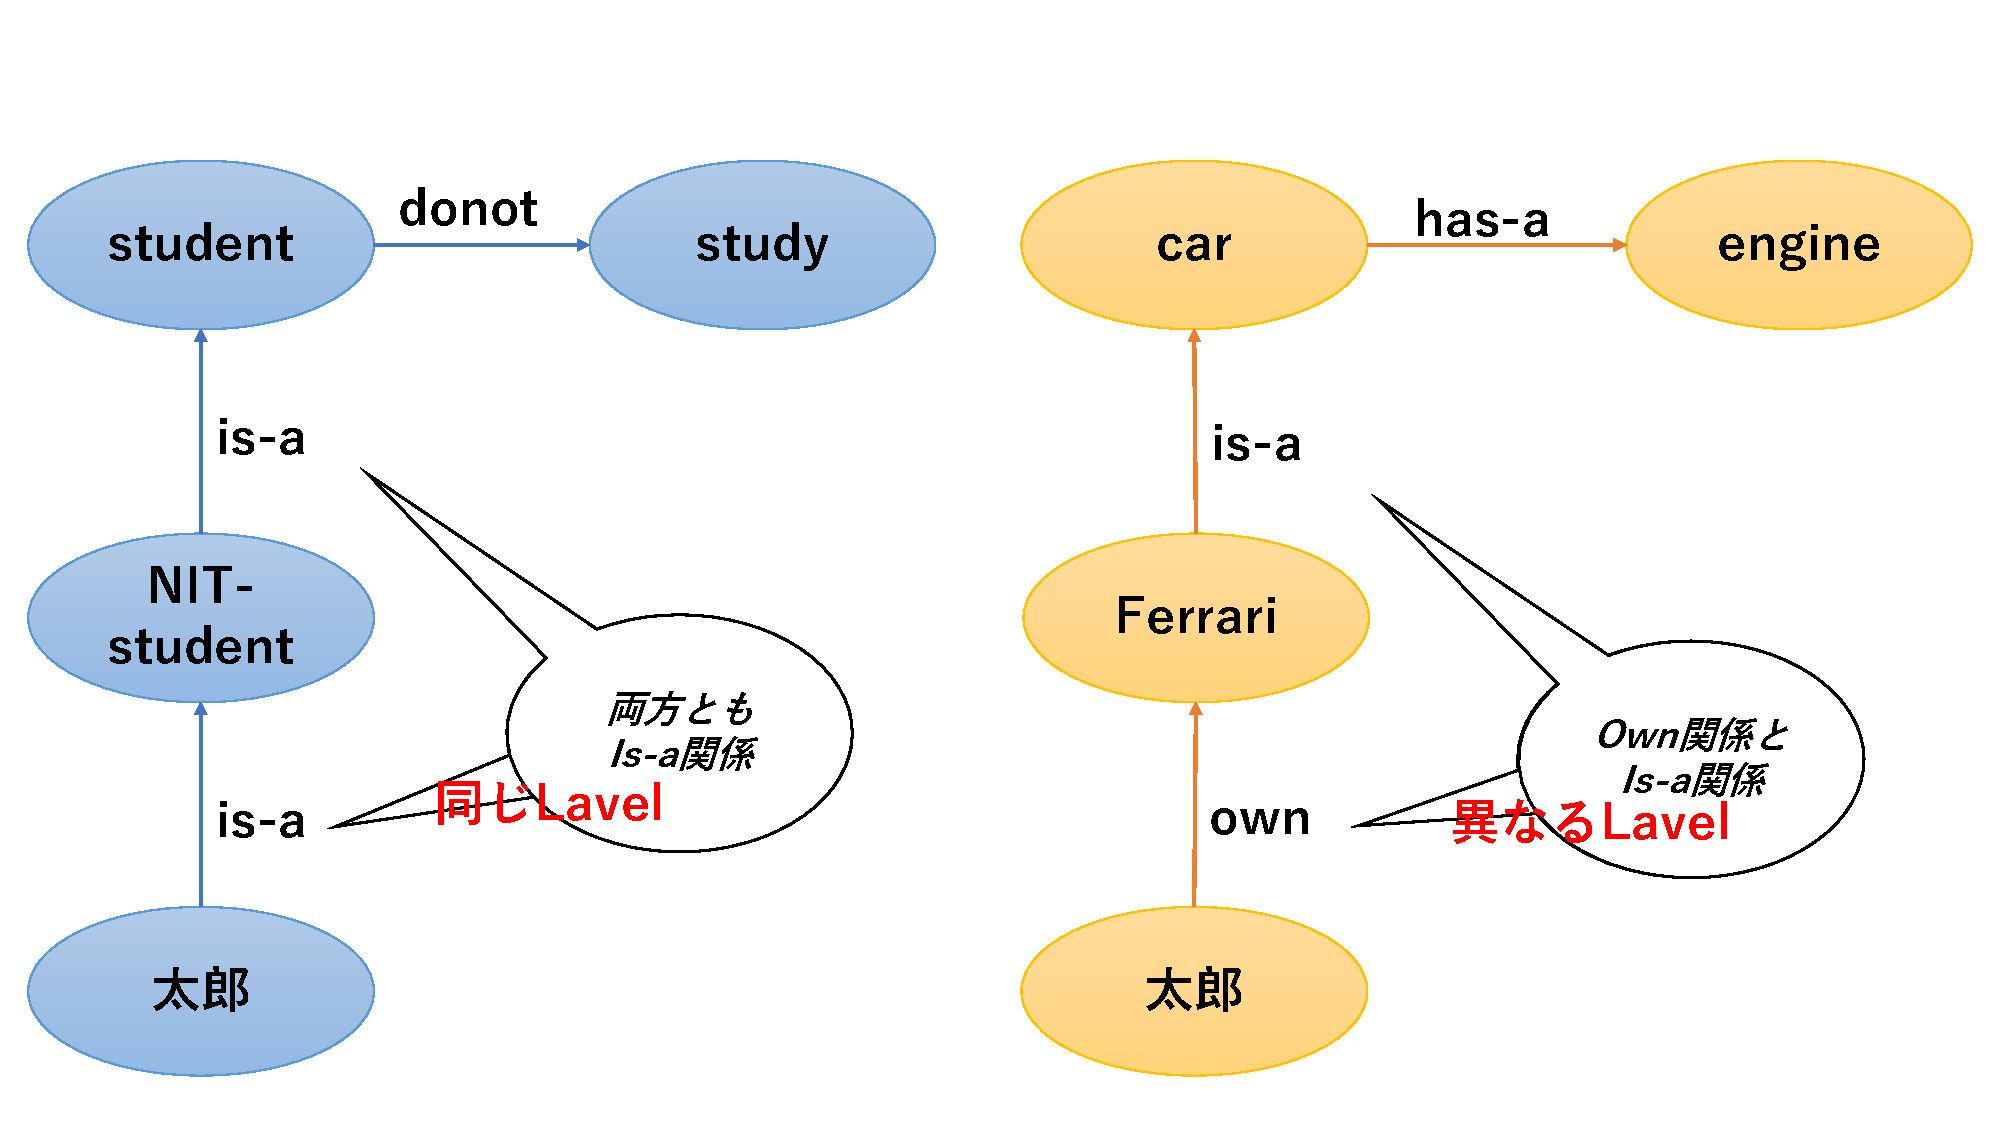
\includegraphics[width = 9cm, pagebox = cropbox, clip]{継承とLabelの対応.pdf}
 \end{center}
 \caption[]{継承とLabelの対応}\label{fig:fig1.1}
\end{figure}

太郎とFerrariのラベル"own"と Ferrariとcarのラベル"is-a"は異なるため, 太郎はcarを持っていることにはならない. 同様に車はエンジンを持つので, つまり太郎はエンジンをもつということは, 文脈上成り立つが, この知識表現ではラベルの違いから成り立たない. その一方で, "太郎は勉強をしない"という文は成り立つ. これは, "is-a"ラベルがNIT-studentもstudentにも成り立ち, 太郎はstudentまでつながれるからである.

また, 知識ベースに登録する際に, "主語(Tail)に応じて動詞(Label)に三単現のsをつけたりつけなかったり変えてはならない. 統一しなければならない"ということもポイントであった. なぜなら上記でも述べたようにあくまでLabelによって関係性が構築されるので, "所有する"という意味でも, "own"と"owns"はどちらかに統一しなければならない. この点が英語における質問応答の難しいところであった.

\section{感想}
課題3-3については, 問題に「難しければ課題2で扱ったような変数を含むパターン (クエリー) でも構わない」とあったので, まずは動くプログラムをということで手法1に取り組んだ. 手法1が済んだので, その知識をベースに手法2にも取り組めた. 時間があればmecabを使った日本語の文章での質問応答も取り組みたかったができなかった. このように段階的に課題を進めれるとかなりやりやすかった.

Javaの使い方は, ググってもいいが, 昔しっかり使い込んだ教科書に立ち戻るのも, また一挙である. 今回は課題3-3で文字列読み込みに用いられたScannerクラスとdo-while文の複数入力プログラムをJava入門の教科書から参照した.

英文での質問を処理する際に, 「a」とか「the」とかの前置詞を取るのがめんどくさかった. 私はあまり英語が得意ではないので, Google翻訳先生に頼り, 前置詞を補完, 処理していった. 前置詞は日本人にとってなじみにくい...

%%%%%%%%%%%%%%%%%%%%%%%%%%%%%%%%%%%%%%%%%%%%%%%%%%%%%%%%%%%%%%%%%%%%%%%%%%%%%%
% 参考文献
\begin{thebibliography}{99}
\bibitem{notty} Javaによる知能プログラミング入門 --著:新谷 虎松 \\
\bibitem{notty} 新・明解 Java 入門 --著:柴田望洋 \\
\bibitem{notty} Java 指定型の読み取り --著:Let's プログラミング \\
\url{https://www.javadrive.jp/start/scanner/index2.html}
\bibitem{notty} Google翻訳 --著:Google \\
\url{https://translate.google.com/?hl=ja}
\end{thebibliography}

\end{document}